\section{El núcleo y la imagen }

\subsection{}

\begin{frame}\frametitle{Núcleo de una transformación lineal}

\begin{alertblock}{\textbf{Observación 1}}
	Si $T:V\to W$ es una transformación lineal, entonces
	\[
		T(\mathbf{0}_{\scalebox{0.4}{V}}) = \mathbf{0}_{\scalebox{0.4}{W}}	
	\]
\end{alertblock}

\begin{block}{\textbf{Definición 1 (Núcleo)}}
	\justifying
	Sea $T:V\to W$ una transformación lineal. El \textbf{\textit{núcleo}} de $T$ es el conjunto de 
	todos los vectores $\mathbf{v}$ en $V$ tales que $T(\mathbf{v}) = \mathbf{0}_{\scalebox{0.4}{W}}$:
	\[
		\text{nu}\ T = \{ \mathbf{v}\in V \mid T(\mathbf{v}) = \mathbf{0}_{\scalebox{0.4}{W}} \}.
	\]
\end{block}


\end{frame}

% ---------------------------------------------------------------------------------------------------

\subsection{}

\begin{frame}\frametitle{Núcleo de una transformación lineal}
		
	\begin{block}{\textbf{Definición 1 (Núcleo)}}
		\justifying
		Sea $T:V\to W$ una transformación lineal. El \textbf{\textit{núcleo}} de $T$ es el conjunto de 
		todos los vectores $\mathbf{v}$ en $V$ tales que $T(\mathbf{v}) = \mathbf{0}_{\scalebox{0.4}{W}}$:
		\[
		\text{nu}\ T = \{ \mathbf{v}\in V \mid T(\mathbf{v}) = \mathbf{0}_{\scalebox{0.4}{W}} \}.
		\]
	\end{block}
	
	\begin{ej}{\textbf{Ejemplo 1}}
		\justifying
		Sea $T:M_{32}\to M_{23}$ la transformación lineal definida por
		\[
		T(A) = A^T.
		\]
		Encuentre el núcleo de $T$.
	\end{ej}
	\textit{Solución.}
	
\end{frame}

% ---------------------------------------------------------------------------------------------------

\subsection{}

\begin{frame}\frametitle{Núcleo de las transformaciones cero e identidad}
	
	\begin{block}{\textbf{Definición 1 (Núcleo)}}
		\justifying
		Sea $T:V\to W$ una transformación lineal. El \textbf{\textit{núcleo}} de $T$ es el conjunto de 
		todos los vectores $\mathbf{v}$ en $V$ tales que $T(\mathbf{v}) = \mathbf{0}_{\scalebox{0.4}{W}}$:
		\[
		\text{nu}\ T = \{ \mathbf{v}\in V \mid T(\mathbf{v}) = \mathbf{0}_{\scalebox{0.4}{W}} \}.
		\]
	\end{block}
	
	
	\begin{ej}{\textbf{Ejemplo 2}}
		\justifying
		Encuentre el núcleo de la \textbf{\textit{transformación cero}} $T:V\to W$ definida por
		\[
		T(\mathbf{v}) = \mathbf{0}_{\scalebox{0.4}{W}}, \quad \text{ para todo } \mathbf{v} \text{ en } V.
		\]
	\end{ej}
	\textit{Solución.}
	
\end{frame}

% ---------------------------------------------------------------------------------------------------

\subsection{}

\begin{frame}\frametitle{Núcleo de las transformaciones cero e identidad}
	
	\begin{block}{\textbf{Definición 1 (Núcleo)}}
		\justifying
		Sea $T:V\to W$ una transformación lineal. El \textbf{\textit{núcleo}} de $T$ es el conjunto de 
		todos los vectores $\mathbf{v}$ en $V$ tales que $T(\mathbf{v}) = \mathbf{0}_{\scalebox{0.4}{W}}$:
		\[
		\text{nu}\ T = \{ \mathbf{v}\in V \mid T(\mathbf{v}) = \mathbf{0}_{\scalebox{0.4}{W}} \}.
		\]
	\end{block}
		
	\begin{ej}{\textbf{Ejemplo 3}}
		\justifying
		Encuentre el núcleo de la \textbf{\textit{transformación identidad}} $T:V\to V$ definida por
		\[
		T(\mathbf{v}) = \mathbf{v}, \quad \text{ para todo } \mathbf{v} \text{ en } V.
		\]
	\end{ej}
	\textit{Solución.}
	
\end{frame}

% ---------------------------------------------------------------------------------------------------

\subsection{}

\begin{frame}\frametitle{Núcleo de una transformación lineal}

\begin{block}{\textbf{Definición 1 (Núcleo)}}
	\justifying
	Sea $T:V\to W$ una transformación lineal. El \textbf{\textit{núcleo}} de $T$ es el conjunto de 
	todos los vectores $\mathbf{v}$ en $V$ tales que $T(\mathbf{v}) = \mathbf{0}_{\scalebox{0.4}{W}}$:
	\[
	\text{nu}\ T = \{ \mathbf{v}\in V \mid T(\mathbf{v}) = \mathbf{0}_{\scalebox{0.4}{W}} \}.
	\]
\end{block}


\begin{ej}{\textbf{Ejemplo 4}}
	\justifying
	Encuentre el núcleo de la transformación lineal $T:\r^3\to \r^3$ definida por
	\[
		T(x,y,z) = (x,y,0).
	\]
\end{ej}
\textit{Solución.}

\end{frame}

% ---------------------------------------------------------------------------------------------------

\subsection{}

\begin{frame}\frametitle{Núcleo de una transformación lineal}
	
	\begin{block}{\textbf{Definición 1 (Núcleo)}}
		\justifying
		Sea $T:V\to W$ una transformación lineal. El \textbf{\textit{núcleo}} de $T$ es el conjunto de 
		todos los vectores $\mathbf{v}$ en $V$ tales que $T(\mathbf{v}) = \mathbf{0}_{\scalebox{0.4}{W}}$:
		\[
		\text{nu}\ T = \{ \mathbf{v}\in V \mid T(\mathbf{v}) = \mathbf{0}_{\scalebox{0.4}{W}} \}.
		\]
	\end{block}
	
	\begin{ej}{\textbf{Ejemplo 5}}
		\justifying
		Encuentre el núcleo de la transformación lineal $T:\r^2\to \r^3$ definida por
		\[
		T(x_1,x_2) = (x_2-2x_1,0,-x_1).
		\]
	\end{ej}
	\textit{Solución.}
	
\end{frame}

% ---------------------------------------------------------------------------------------------------

\subsection{}

\begin{frame}\frametitle{Núcleo de una transformación lineal}

\begin{block}{\textbf{Definición 1 (Núcleo)}}
	\justifying
	Sea $T:V\to W$ una transformación lineal. El \textbf{\textit{núcleo}} de $T$ es el conjunto de 
	todos los vectores $\mathbf{v}$ en $V$ tales que $T(\mathbf{v}) = \mathbf{0}_{\scalebox{0.4}{W}}$:
	\[
	\text{nu}\ T = \{ \mathbf{v}\in V \mid T(\mathbf{v}) = \mathbf{0}_{\scalebox{0.4}{W}} \}.
	\]
\end{block}


\begin{ej}{\textbf{Ejemplo 6}}
	\justifying
	Encuentre el núcleo de la transformación lineal $T:\r^3\to \r^2$ definida por $T(\mathbf{x})=A\mathbf{x}$,
	donde
	\[
	A = 
	\left(
	\begin{array}{@{\hspace{0.3\tabcolsep}}r@{\hspace{1.2\tabcolsep}}r@{\hspace{1.2\tabcolsep}}r@{\hspace{0.3\tabcolsep}}}
	 1 & -1 & -2 \\[1mm]
	-1 & 2 & 3
	\end{array}
	\right).
	\]
\end{ej}
\textit{Solución.}

\end{frame}

% ---------------------------------------------------------------------------------------------------

\subsection{}

\begin{frame}\frametitle{Propiedades del núcleo}

\begin{prop}{\textbf{Propiedad 1}}
	\justifying
	El núcleo $\text{nu}\ T$ de una transformación lineal $T:V\to W$ es un subespacio vectorial de $V$.
\end{prop}	

\end{frame}

% ---------------------------------------------------------------------------------------------------

\subsection{}

\begin{frame}\frametitle{Propiedades del núcleo}
	
	\begin{prop}{\textbf{Propiedad 2}}
		\justifying
		Sea $A$ una matriz $m\times n$ y $T:\r^n\to \r^m$ la transformación lineal definida por
		\[
		T(\mathbf{x})=A\mathbf{x}.
		\]
		Entonces el núcleo de $T$ es igual al espacio solución del sistema 
		\[
		A\mathbf{x}=\mathbf{0}.
		\] 
		Es decir, el núcleo de $T$ es igual al \textbf{\textit{espacio nulo}} de $A$:
		\[
		\text{nu}\, T = N_A = \{ \mathbf{x}\in\r^n \mid A\mathbf{x} = \mathbf{0} \}
		\]
	\end{prop}	
	
\end{frame}


% ---------------------------------------------------------------------------------------------------

\subsection{}

{\nologo
\begin{frame}\frametitle{Imagen de una transformación lineal}

\vspace{-3mm}
\begin{block}{\textbf{Definición 2 (Imagen)}}
	\justifying
	Sea $T:V\to W$ una transformación lineal. La \textbf{\textit{imagen}} de $T$ es el conjunto de 
	todos los vectores $\mathbf{w}$ en $W$ que son imágenes de vectores en $V$. Es decir,
	\[
	\text{im}\ T = \{ T(\mathbf{v}) \mid \mathbf{v}\in V \}.
	\]
\end{block}

\vspace{-1mm}

\begin{prop}{\textbf{Propiedad 3}}
	\justifying
	La imagen $\text{im}\ T$ de una transformación lineal $T:V\to W$ es un subespacio vectorial de $W$.
\end{prop}	

\vspace{-1mm}

\begin{alertblock}{\textbf{Observación 2}}
	Sea $T:V \to W$ una transformación lineal.
	
	\vspace{-2mm}
	\begin{multicols}{2}
		\begin{figure}		
			\centering
			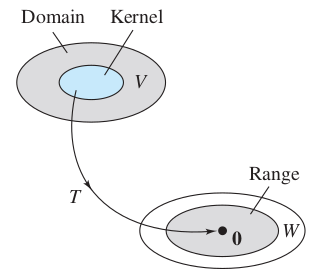
\includegraphics[width=0.25\textwidth]{imagenes/espacios}
		\end{figure}
				
		\begin{enumerate}
			\item[\labelname{$a$}] $\text{nu}\ T$ es un subespacio de $V$.\\[6mm]
			\item[\labelname{$b$}] $\text{im}\ T$ es un subespacio de $W$.
		\end{enumerate}
	\end{multicols}

\end{alertblock}

\end{frame}
}

%%------------------------------------------------------------------------------------------------------

\subsection{}

{\nologo
\begin{frame}\frametitle{Imagen de una transformación lineal}

\begin{alertblock}{\textbf{Observación 2}}
Sea $A$ una matriz $m\times n$ y $T:\r^n\to \r^m$ la transformación lineal 
\[
	T(\mathbf{x})=A\mathbf{x}.
\]
\[
%{\color{blue}
	A\mathbf{x} =\hspace{-1mm} 
	\left(
	\begin{array}{@{\hspace{0.1\tabcolsep}}c@{\hspace{1\tabcolsep}}c@{\hspace{1\tabcolsep}}c@{\hspace{1\tabcolsep}}c@{\hspace{0.1\tabcolsep}}}
	a_{11} & a_{12} & \cdots & a_{1n} \\[1mm]
	a_{21} & a_{22} & \cdots & a_{2n} \\[1mm]
	\vdots & \vdots &        & \vdots \\[0mm]
	a_{m1} & a_{m2} & \cdots & a_{mn} \\[1mm]
	\end{array}
	\right)
	\hspace{-1.5mm}
	\left(
	\begin{array}{@{\hspace{0.1\tabcolsep}}c@{\hspace{0.1\tabcolsep}}}
	x_{1} \\[1mm]
	x_{2} \\[1mm]
	\vdots \\[0mm]
	x_{m} \\[1mm]
	\end{array}
	\right)%}\ 
	\hspace{-1mm} = 
	x_1\hspace{-1mm}
	\left(
	\begin{array}{@{\hspace{0.1\tabcolsep}}c@{\hspace{0.1\tabcolsep}}}
	a_{11} \\[1mm]
	a_{21} \\[1mm]
	\vdots \\[0mm]
	a_{m1} \\[1mm]
	\end{array}
	\right)\ 
	+\ 
	%x_2
	%\left(
	%\begin{array}{@{\hspace{0.1\tabcolsep}}c@{\hspace{0.1\tabcolsep}}}
	%a_{12} \\[1mm]
	%a_{22} \\[1mm]
	%\vdots \\[0mm]
	%a_{m2} \\[1mm]
	%\end{array}
	%\right)\ 
	%+\ 
	\cdots\ 
	+\ 
	x_n\hspace{-1mm}
	\left(
	\begin{array}{@{\hspace{0.1\tabcolsep}}c@{\hspace{0.1\tabcolsep}}}
	a_{1n} \\[1mm]
	a_{2n} \\[1mm]
	\vdots \\[0mm]
	a_{mn} \\[1mm]
	\end{array}
	\right)
	=
%	{\color{red}
		\left(
		\begin{array}{@{\hspace{0.1\tabcolsep}}c@{\hspace{0.1\tabcolsep}}}
		b_{1} \\[1mm]
		b_{2} \\[1mm]
		\vdots \\[0mm]
		b_{m} \\[1mm]
		\end{array}
		\right)
%	}
\]

\[
\mathbf{b}\in \text{im}\ T \quad \Longleftrightarrow \quad
T(\mathbf{x})=\mathbf{b} \quad \Longleftrightarrow \quad 
A\mathbf{x}=\mathbf{b} \quad \Longleftrightarrow \quad 
\mathbf{b}\in C_A
\]
\end{alertblock}

\begin{prop}{\textbf{Propiedad 4}}
	\justifying
	Sea $A$ una matriz $m\times n$ y $T:\r^n\to \r^m$ la transformación lineal $T(\mathbf{x})=A\mathbf{x}$.
	Entonces la \textbf{\textit{imagen}} de $T$ es igual al \textbf{\textit{espacio generado por las columnas}} de $A$. Es decir, 
	\[
		\text{im}\ T = C_A.
	\]
\end{prop}	

\end{frame}
}

% ---------------------------------------------------------------------------------------------------

\subsection{}

\begin{frame}%\frametitle{Imagen de una transformación lineal}

%\begin{prop}{\textbf{Propiedad 4}}
%	\justifying
%	Sea $A$ una matriz $m\times n$ y $T:\r^n\to \r^m$ la transformación lineal $T(\mathbf{x})=A\mathbf{x}$.
%	Entonces la \textbf{\textit{imagen}} de $T$ es igual al \textbf{\textit{espacio generado por las columnas}} de $A$. Es decir, 
%	\[
%	\text{im}\ T = C_A.
%	\]
%\end{prop}	

\begin{ej}{\textbf{Ejemplo 7}}
	\justifying
	Considere la transformación lineal $T:\r^5\to \r^4$ definida por $T(\mathbf{x})=A\mathbf{x}$,
	donde
	\[
	A = 
	\left(
	\begin{array}{@{\hspace{0.3\tabcolsep}}r@{\hspace{1.5\tabcolsep}}r@{\hspace{1.5\tabcolsep}}r@{\hspace{1.5\tabcolsep}}r@{\hspace{1.5\tabcolsep}}r@{\hspace{0.3\tabcolsep}}}
	 1 & \phantom{-}2 &  0 & \phantom{-}1 & -1 \\[1mm]
	 2 & 1 &  3 & 1 &  0 \\[1mm]
	-1 & 0 & -2 & 0 &  1 \\[1mm]
	 0 & 0 &  0 & 2 &  8 
	\end{array}
	\right).
	\]
	Encuentre una base para $\text{im}\ T$.
\end{ej}
\textit{Solución.}

\end{frame}

% ---------------------------------------------------------------------------------------------------

\subsection{}

{\nologo
\begin{frame}\frametitle{Rango y nulidad de una transformación lineal}

\vspace{-2mm}
\begin{defi}{\textbf{Definición 3 (Rango y nulidad)}}\justifying
	Sea $T:V\to W$ una transformación lineal.
	\begin{enumerate}
		\item[\labelname{$a$}] A la dimensión del núcleo de $T$ se le llama la \textbf{\textit{nulidad}} de $T$ 
		y se la denota por $\nu(T)$:
		\[
			\nu(T) = \dim \text{nu}\, T.
		\]
		\item[\labelname{$b$}] A la dimensión de la imagen de $T$ se le llama el \textbf{\textit{rango}} de $T$ 
		y se la denota por $\rho(T)$:
		\[
		\rho(T) = \dim \text{im}\, T.
		\]
	\end{enumerate}
\end{defi}	

\begin{alertblock}{\textbf{Observación 1}}\justifying
	Si $A$ una matriz $m\times n$ y $T:\r^n\to \r^m$ es la transformación lineal $T(\mathbf{x})=A\mathbf{x}$, entonces:
	\begin{enumerate}
		\item[\labelname{$a$}] $\rho(T) = \dim \text{im}\, T = \dim C_A = \rho(A)$.
		\item[\labelname{$b$}] $\nu(T) = \dim \text{nu}\, T = \dim N_A = \nu(A)$.
		\item[\labelname{$c$}] $\rho(A) + \nu(A) = \text{ número de columnas de } A = n$.
		\item[\labelname{$d$}] $\rho(T) + \nu(T) = n = \dim \r^n$.
	\end{enumerate}

\end{alertblock}

\end{frame}
}
% ---------------------------------------------------------------------------------------------------

\subsection{}

{\nologo
\begin{frame}\frametitle{Rango y nulidad de una transformación lineal}

\vspace{-2mm}

\begin{defi}{\textbf{Definición 3 (Rango y nulidad)}}\justifying
	Sea $T:V\to W$ una transformación lineal.
	\begin{enumerate}
		\item[\labelname{$a$}] A la dimensión del núcleo de $T$ se le llama la \textbf{\textit{nulidad}} de $T$ y se denota por $\nu(T)$:
		\[
		\nu(T) = \dim \text{nu}\, T.
		\]
		\item[\labelname{$b$}] A la dimensión de la imagen de $T$ se le llama el \textbf{\textit{rango}} de $T$ y se denota por $\rho(T)$:
		\[
		\rho(T) = \dim \text{im}\, T.
		\]
	\end{enumerate}
\end{defi}	

\vspace{-1mm}

\begin{prop}{\textbf{Propiedad 5}}
	\justifying
	Sea $T:V\to W$ una transformación lineal definida en un espacio vectorial $V$ de dimensión $n$. Entonces
	\[
		\rho(T) + \nu(T) = n = \dim V.
	\]
\end{prop}	

\vspace{-1mm}

\begin{alertblock}{\textbf{Observación 1}}

\begin{center}
	``dimensión de la imagen + dimensión del núcleo = dimensión del dominio''
\end{center}
\end{alertblock}

\end{frame}
}

% ---------------------------------------------------------------------------------------------------

\subsection{}

\begin{frame}%\frametitle{Determinación del rango y la nulidad de una transformación lineal}

\begin{prop}{\textbf{Propiedad 5}}
	\justifying
	Sea $T:V\to W$ una transformación lineal definida en un espacio vectorial $V$ de dimensión $n$. Entonces
	\[
	\rho(T) + \nu(T) = n = \dim V.
	\]
\end{prop}	

\begin{ej}{\textbf{Ejemplo 7}}
	\justifying
	Sea $T:\r^3\to \r^3$ la transformación lineal definida por 
	\[
	A = 
	\left(
	\begin{array}{@{\hspace{0.5\tabcolsep}}r@{\hspace{1.5\tabcolsep}}r@{\hspace{1.5\tabcolsep}}r@{\hspace{0.5\tabcolsep}}}
	1 & \phantom{-}0 & -2 \\[1mm]
	0 & 1 &  1  \\[1mm]
	0 & 0 &  0 
	\end{array}
	\right).
	\]
	Encuentre el rango y la nulidad de $T$.
\end{ej}
\textit{Solución.}

\end{frame}

% ---------------------------------------------------------------------------------------------------

\subsection{}

\begin{frame}\frametitle{Determinación del rango y la nulidad de una transformación lineal}

%\begin{prop}{\textbf{Propiedad 5}}
%	\justifying
%	Sea $T:V\to W$ una transformación lineal definida en un espacio vectorial $V$ de dimensión $n$. Entonces
%	\[
%	\rho(T) + \nu(T) = n = \dim V.
%	\]
%\end{prop}	

\begin{ej}{\textbf{Ejemplo 8}}
	\justifying
	Sea $T:\r^5\to \r^7$ una transformación lineal.
	\begin{enumerate}
		\item[\labelname{$a$}] Encuentre la dimensión del núcleo de $T$ si el rango es $2$.
		\item[\labelname{$b$}] Encuentre el rango de $T$ si la nulidad de $T$ es 4.
		\item[\labelname{$c$}] Encuentre el rango de $T$ si $\text{nu}\,T=\{\mathbf{0}\}$.
	\end{enumerate}
\end{ej}
\textit{Solución.}

\end{frame}
